\documentclass[11pt]{amsart}
\usepackage{geometry}                % See geometry.pdf to learn the layout options. There are lots.
\geometry{letterpaper}                   % ... or a4paper or a5paper or ... 
%\geometry{landscape}                % Activate for for rotated page geometry
%\usepackage[parfill]{parskip}    % Activate to begin paragraphs with an empty line rather than an indent
\usepackage{graphicx}
\usepackage{amssymb}
\usepackage{python}
\usepackage{epstopdf}
\usepackage{listings}
\usepackage{color}
 
\definecolor{codegreen}{rgb}{0,0.6,0}
\definecolor{codegray}{rgb}{0.5,0.5,0.5}
\definecolor{codepurple}{rgb}{0.58,0,0.82}
\definecolor{backcolour}{rgb}{0.95,0.95,0.92}
 
\lstdefinestyle{mystyle}{
    %backgroundcolor=\color{backcolour},   
    commentstyle=\color{codegreen},
    keywordstyle=\color{magenta},
    numberstyle=\tiny\color{codegray},
    stringstyle=\color{codepurple},
    basicstyle=\footnotesize,
    breakatwhitespace=false,         
    breaklines=true,                 
    captionpos=b,                    
    keepspaces=true,                 
    numbers=left,                    
    numbersep=5pt,                  
    showspaces=false,                
    showstringspaces=false,
    showtabs=false,                  
    tabsize=2
}
 
\lstset{style=mystyle}
\DeclareGraphicsRule{.tif}{png}{.png}{`convert #1 `dirname #1`/`basename #1 .tif`.png}

\title{Homework 7}
\author{Carter Rhea}
\date{\today}                                           

\begin{document}
\maketitle
\section{Problem 1}
Statement: Consider the following function
$$f(x)=e^{2x} \ \ \ x \in (-1,1) $$
Evaluate the integral of the function in its given interval using Gauss quadrature with 1, 2,
3, and 5 integration points. Plot the absolute value of the error between the approximation
and the true solution versus the number of integration points.
\\ \\
Solution:
\begin{center}
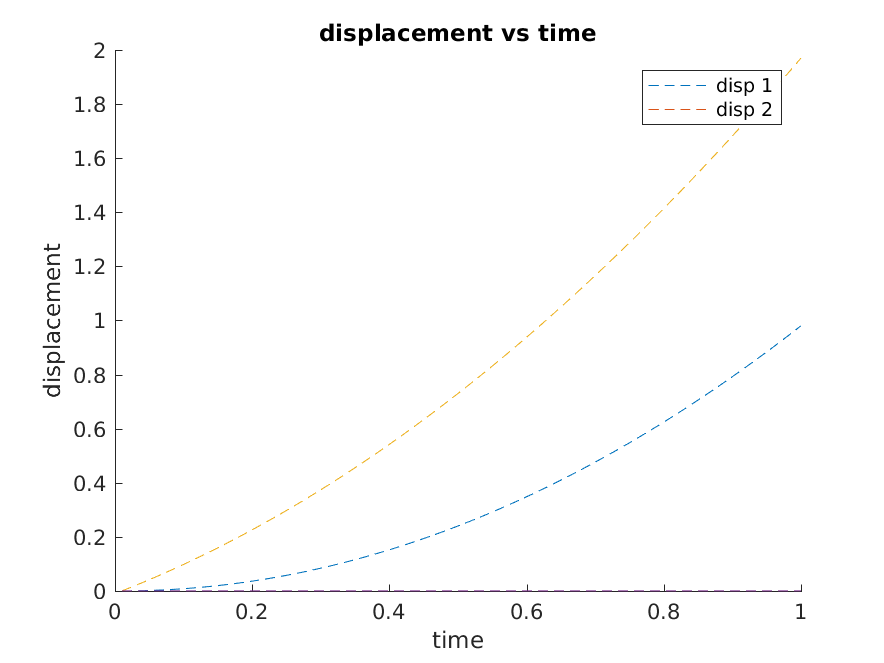
\includegraphics[scale=0.5]{/Users/crhea/Documents/Grad/Math/530_FEM/HW7/problem1.png}
\end{center}
\pagebreak
\section{Problem 2}
Statement: What is the lowest Gauss quadrature integration rule (n x n) that can be used
to fully integrate the stiffness matrix of a (solid mechanics) Q9 element (assume the
element is undistorted)? Show some derivations to support your answer.\\ \\
Solution:\\
For a $Q9$ element, each of the shape functions will be $up \ to \ a$ quadratic, both in the $x$ and $y$ direction. We know that for a polynomial of order $p$ we need the number of quadrature integration points -- $N_{ip}$ -- to satisfy the following inequality:
$$p \leq 2N_{ip}-1 $$
\\
Hence since we have a third order polynomial $(p=3)$, $N_{ip}$ must be equal to 2 or more!\\
Note that the third order term might be of the following form $x^2,y^2$.\\


\section{Problem 3}
Statement: Compute the determinant of the Jacobian matrix for the two mapped
elements shown below using the shape functions defined over the given parent element.
The determinant of the Jacobian matrix becomes negative when the numbering of the
mapped element is clockwise. Comment on the implication of having a negative Jacobian
in a finite element formulation. \\ \\ 
Solution:\\
For the first drawn element with normal nodal numbering (i.e. counter-clockwise starting in the bottom left corner), the shape functions are thus:
$$N_1(\xi,\eta)  = \frac{1}{4}(1-\xi)(1-\eta)$$
$$N_2(\xi,\eta)  = \frac{1}{4}(1+\xi)(1-\eta)$$
$$N_3(\xi,\eta)  = \frac{1}{4}(1+\xi)(1+\eta)$$
$$N_4(\xi,\eta)  = \frac{1}{4}(1-\xi)(1+\eta)$$

The main difference is the ordering of the nodal values.  \\
For part A we use $([-a,-b],[a,-b],[a,b],[-a,b])$ and for part B we use $([-a,-b],[-a,b],[a,b],[a,-b])$.

Note the following relations:
$$[G] = [\nabla N1 \ \ \nabla N2 \ \ \nabla N3 \ \ \nabla N4]$$
\begin{equation*}
[C] = 
  \begin{bmatrix}
    x_1&y_1\\
    x_2&y_2\\
    x_3&y_3\\
    x_4&y_4
  \end{bmatrix}
\end{equation*}

$$[J] = [G][C] $$

In a python script I ran the actual calculations for $[J]$ because that would be a real pain to type in \LaTeX...



\begin{lstlisting}[language=Python]
from sympy import symbols, diff
from sympy.matrices import Matrix
import numpy as np
x, y = symbols('x y')
a , b = symbols('a b')
#first element
N1_1 = (1/(4*a*b))*(a-x)*(b-y)
N1_2 = (1/(4*a*b))*(a+x)*(b-y)
N1_3 = (1/(4*a*b))*(a+x)*(b+y)
N1_4 = (1/(4*a*b))*(a-x)*(b+y)

N1=[N1_1, N1_2, N1_3, N1_4]
Coord_mat1 = Matrix(([-a,-b],[a,-b],[a,b],[-a,b]))

Coord_mat2 = Matrix(([-a,-b],[-a,b],[a,b],[a,-b]))

def Det_jac(N,Coord_mat):
    G = Matrix(([0,0,0,0],[0,0,0,0]))
    for i in range(4):
        G[0,i] = diff(N[i] ,x)
        #print(G[0,i])
        G[1,i] = diff(N[i] ,y)
        #print(G[1,i])
    ##now jacobian
    J = G*Coord_mat
    return J.det()

print(Det_jac(N1,Coord_mat1))
print(Det_jac(N1,Coord_mat2))


\end{lstlisting}

The output is simply $1 , -1$ which is exactly what we want! The negative Jacobian indicates the direction (clockwise) of the ordering.

\

\section{Problem 4}
Part c: stiffness matrix \\
\begin{center}
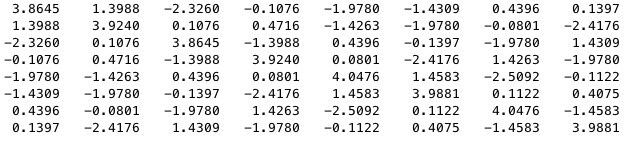
\includegraphics[scale=0.5]{/Users/crhea/Documents/Grad/Math/530_FEM/HW7/HW_7_4_c.png}
\end{center}

Part d: Load Vector \\
\begin{center}
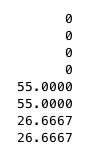
\includegraphics[scale=0.5]{/Users/crhea/Documents/Grad/Math/530_FEM/HW7/HW_7_4_d.png}
\end{center}

\section{Problem 5}
Show that the area of any mapped four-node (bilinear) quad element can be
obtained exactly by using one integration point. That is, you need to show that the
integral
$$A^e = \int_{A^e}dA $$
can be computed exactly with a one-point Gauss quadrature rule.\\
Solution:\\
Since we are looking at the area of a mapped element, the parent element will have an area of 4 (since the side lengths are 2 each). Hence we want to check that we get $A=4$ if we calculate area using Gaussian Quadratrue.
By definition, 
$$A = \int_{A^e}1*dA = \int \int 1 dx dy$$
So if we allow $f(x)=1$ and apply gaussian quadrature with n=1 (hence $x=0 \ , \ w=2$, we have
$$\sum_{i=1}^1 \sum_{i=1}^1 f(x)*w_ip*w_ip = \sum_{i=1}^1 \sum_{i=1}^1 1*2*2 = 4$$
Hence the area is accurately calculated using one point GQ.












\end{document}  